\begin{figure}[H]
\centering
\resizebox{1.0\textwidth}{!}{%
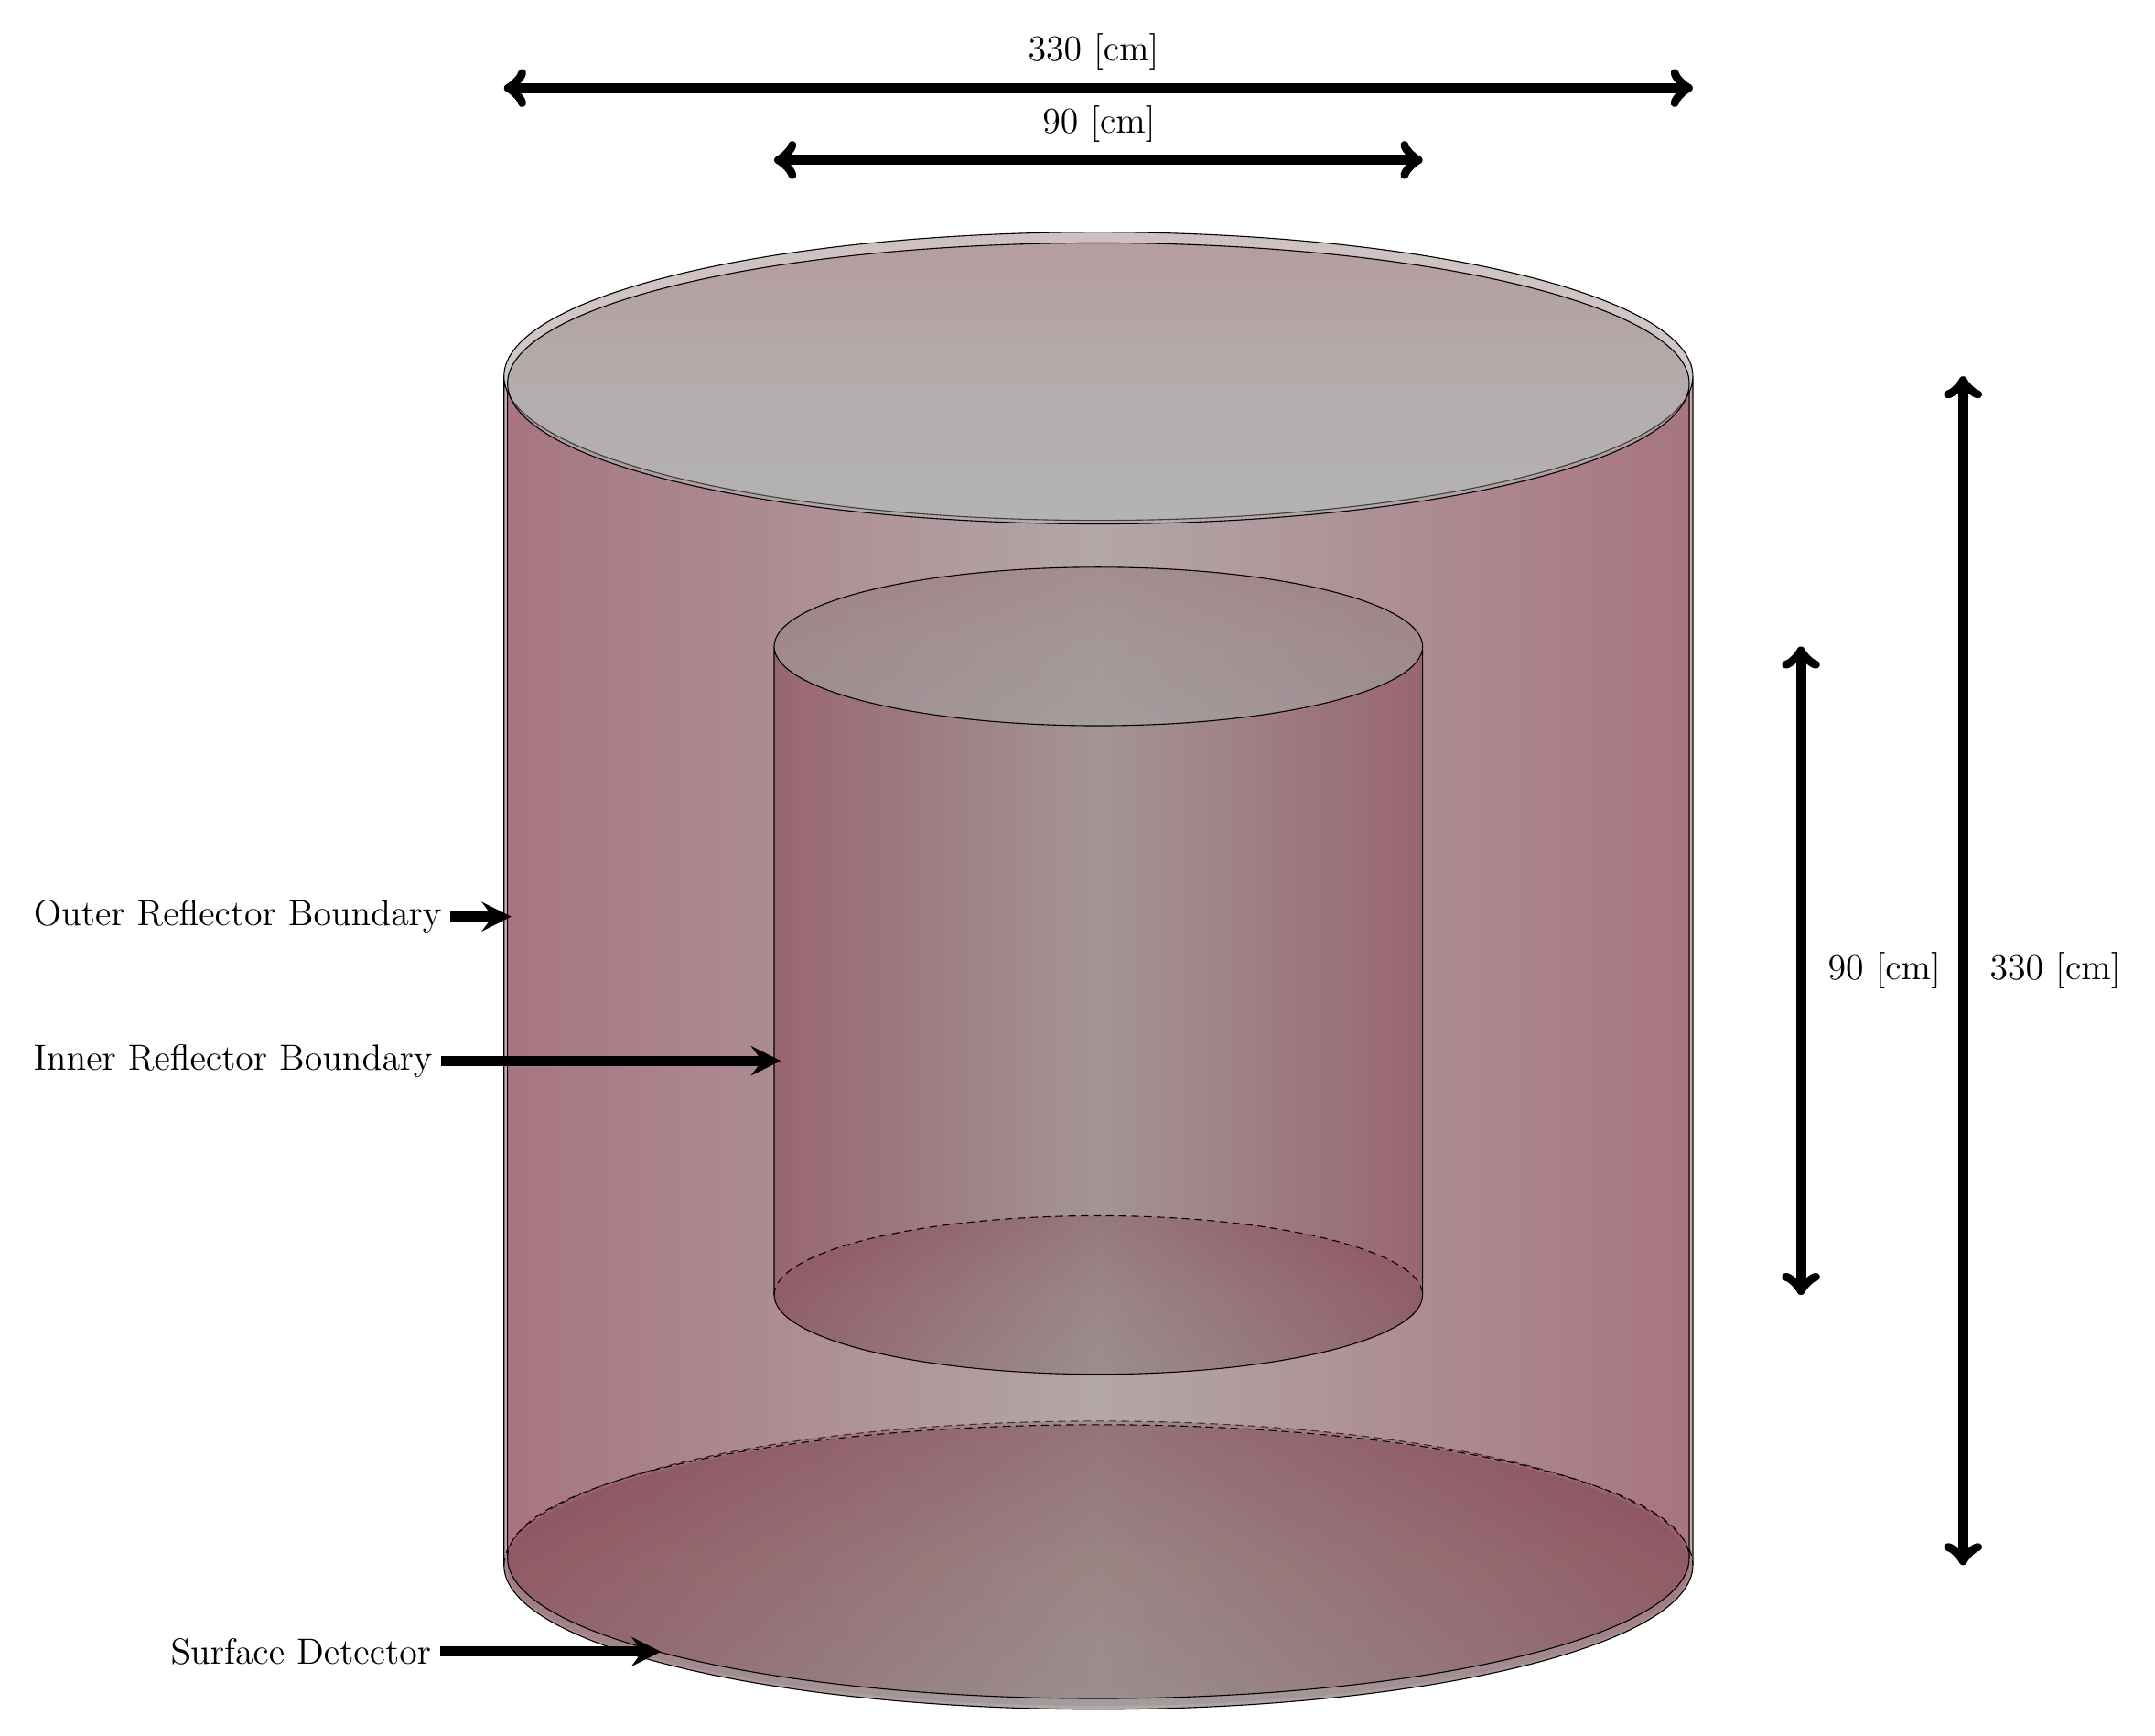
\begin{tikzpicture}
\fill[top color=pink!50!purple,bottom color=pink!10,middle color=pink,shading=axis,opacity=0.25] (0,0) circle (8.25cm and 2.0cm);
\fill[left color=pink!50!purple,right color=pink!50!purple,middle color=pink!50,shading=axis,opacity=0.25] (8.25,0) -- (8.25,16.5) arc (360:180:8.25cm and 2.0cm) -- (-8.25,0) arc (180:360:8.25cm and 2.0cm);
\fill[top color=pink!90!,bottom color=pink!2,middle color=pink!30,shading=axis,opacity=0.25] (0,16.5) circle (8.25cm and 2.0cm);
\draw (-8.25,16.5) -- (-8.25,0) arc (180:360:8.25cm and 2.0cm) -- (8.25,16.5) ++ (-8.25,0) circle (8.25cm and 2.0cm);
\draw[densely dashed] (-8.25,0) arc (180:0:8.25cm and 2.0cm);

\fill[top color=pink!50!purple,bottom color=pink!10,middle color=pink,shading=axis,opacity=0.25] (0,0.0) circle (8.2cm and 1.95cm);
\fill[left color=pink!50!purple,right color=pink!50!purple,middle color=pink!50,shading=axis,opacity=0.25] (8.2,0.1) -- (8.2,16.4) arc (360:180:8.2cm and 1.95cm) -- (-8.2,0.1) arc (180:360:8.2cm and 1.95cm);
\fill[top color=pink!90!,bottom color=pink!2,middle color=pink!30,shading=axis,opacity=0.25] (0,16.4) circle (8.2cm and 1.95cm);
\draw (-8.2,16.3) -- (-8.2,0.1) arc (180:360:8.2cm and 1.95cm) -- (8.2,16.3) ++ (-8.2,0.1) circle (8.2cm and 1.95cm);
\draw[densely dashed] (-8.2,0.1) arc (180:0:8.2cm and 1.85cm);

\fill[top color=pink!50!purple,bottom color=pink!10,middle color=pink,shading=axis,opacity=0.25] (0,3.75) circle (4.5cm and 1.1cm);
\fill[left color=pink!50!purple,right color=pink!50!purple,middle color=pink!50,shading=axis,opacity=0.25] (4.5,3.75) -- (4.5,12.75) arc (360:180:4.5cm and 1.1cm) -- (-4.5,3.75) arc (180:360:4.5cm and 1.1cm);
\fill[top color=pink!90!,bottom color=pink!2,middle color=pink!30,shading=axis,opacity=0.25] (0,12.75) circle (4.5cm and 1.1cm);
\draw (-4.5,12.75) -- (-4.5,3.75) arc (180:360:4.5cm and 1.1cm) -- (4.5,12.75) ++ (-4.5,3.75) (0,12.75) circle (4.5cm and 1.1cm);
\draw[densely dashed] (-4.5,3.75) arc (180:0:4.5cm and 1.1cm);

\node [anchor=west] (out-ref) at (-14.9, 9) {\Large Outer Reflector Boundary};
\node [anchor=west] (in-ref) at (-14.9, 7) {\Large Inner Reflector Boundary};
\node [anchor=west] (det) at (-13, -1.2) {\Large Surface Detector};

\draw [-stealth, line width=4pt, black] (out-ref) -- ++(3.8,0);
\draw [-stealth, line width=4pt, black] (in-ref) -- ++(7.6,0);
\draw [-stealth, line width=4pt, black] (det) -- ++(5.0,0);

\draw [-stealth, <->, line width=4pt, black] ++(-8.25,20.5) -- ++(16.5,0);
\draw [-stealth, <->, line width=4pt, black] ++(12,0) -- ++(0,16.5);

\node [anchor=west] (out-h) at (12.25, 8.25) {\Large 330 [cm]};
\node [anchor=west] (out-d) at (-1.1, 21.0) {\Large 330 [cm]};

\draw [-stealth, <->, line width=4pt, black] ++(-4.5,19.5) -- ++(9,0);
\draw [-stealth, <->, line width=4pt, black] ++(9.75,3.75) -- ++(0,9.0);

\node [anchor=west] (in-h) at (10.0, 8.25) {\Large 90 [cm]};
\node [anchor=west] (in-d) at (-0.9, 20.0) {\Large 90 [cm]};

\end{tikzpicture}
 }%
\caption{Detector Placement Inside Reflector in Sangamon200 and Sangamon20}
\label{fig:det-place}

\end{figure}
